\chapter{Marco Te\'orico}
\label{cap:preliminares}

\section{Redes Neuronales Artificiales}
\label{intro:redes_neuronales}

Con $n$ entradas en el nodo desde $x_1$ hasta $x_n$ y $\varphi$ la funci\'on de activaci\'on. La salida del nodo n\'umero $j$ es:

\vspace*{0.5cm}

\begin{equation}
y_j = \varphi (\displaystyle\sum_{j=i}^{n} w_{ji} x_i + b_j)
\label{eq:output_network}
\end{equation}

\vspace*{0.5cm}  % espacio entre párrafos 

\begin{figure}[ht]
  \centering
  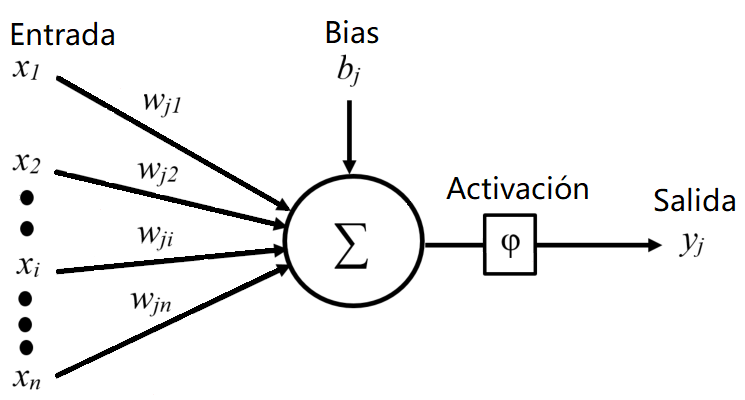
\includegraphics[scale=0.40]{images/neuron_unit_sp.png}
  \caption[Nodo Artificial unitario]{Nodo artificial unitario que imita la estructura cerebral. Su funci\'on es aprender y es un elemento b\'asico de aprendizaje.}
  \label{fig:rna_neuron}
\end{figure}

\clearpage
\section{Funciones de Activaci\'on}
\label{intro:activations}

\subsection{Sigmoide}

Tambi\'en se conoce como funci\'on de activaci\'on log\'istica. Toma un n\'umero de valor real y lo acota en un rango entre 0 y 1. Tambi\'en se usa en la capa de salida donde el objetivo final es predecir una probabilidad. Convierte grandes números negativos en 0 y grandes números positivos en 1. Matem\'aticamente se representa como:

\begin{equation}
\sigma(x) = \frac{1}{1+\mathrm{e}^{-x}}
\label{eq:sigmoide}
\end{equation}

\noindent y su derivada:

\begin{equation}
\frac{\partial}{\partial x} \sigma(x) = \sigma(x)(1-\sigma(x))
\label{eq:sigmoide_derivada}
\end{equation}

\vspace*{0.5cm}

\subsection{LeakyReLU}
\label{leakyrelu_title}

\begin{equation}
\frac{\partial}{\partial x} z(x) = 
\begin{cases}
1   & x > 0 \\
0.1 & x < 0
\end{cases} \label{eq:leaky_derivate}
\end{equation}


\section{M\'etodos de Optimizaci\'on}

\subsection{Descenso del Gradiente Estoc\'astico}

\begin{equation}
W_{t+1} = W_t - \alpha \nabla f(W_t)
\label{eq:sgd}
\end{equation}

\vspace*{0.3cm}

donde $\alpha$ es la tasa de aprendizaje y $\nabla f(W_t)$ es el gradiente (o derivada) de la funci\'on de p\'erdida con respecto de $W$.


\section{Propagaci\'on hacia atr\'as (\emph{Backpropagation})}

Es una t\'ecnica utilizada para realizar eficientemente el descenso del gradiente en una red neuronal \citep{10.5555/65669.104451}.


\section{M\'aquinas de Soporte Vectorial (\emph{support-vector machine})}
\label{intro:svm}

Las M\'aquinas de Soporte Vectorial (\emph{SVM}) son de los algoritmos m\'as populares en Machine Learning. Estos suelen utilizarse en problemas de clasificaci\'on, regresi\'on, e incluso detecci\'on de valores at\'ipicos (\emph{outliers}). El m\'etodo de soporte vectorial fue presentado por Boser, Guyon y Vapnik \citep{boser1992} en la Conferencia ACM de Teoría del Aprendizaje Computacional (COLT92).

\vspace*{0.5cm}

La idea de construir un hiperplano separador \'optimo en un contexto no-param\'etrico, desarrollado por Vapnik y Chervonenkis \citep{Vapnik:1964} y por Cover \citep{4038449}.


\section{Redes Neuronales Convolucionales (\emph{CNN})}
\label{intro:cnns}


\subsection{Capas Convolucionales}


\section{Arquitecturas Comunes}

\subsection{YOLO: You Only Look Once}
\label{teo:yolo}

YOLO fue presentado en el 2016 como un nuevo enfoque para la detecci\'on de objetos. En vez de re-utilizar clasificadores para realizar la detecci\'on, este enmarca la detecci\'on de objectos como un problema de regresi\'on de cajas delimitadores (\emph{bounding box}) espacialmente separadas con una probabilidad asociada. Solo una red neuronal predice cajas delimitadores y probabilidades de las clases directamente desde la imagen completa en una sola evaluaci\'on. De esta manera, esta arquitectura se deshace de complejos diagramas de flujo (\emph{pipelines}) y la hace extremadamente r\'apida \citep{redmon2016look}.

\vspace*{0.5cm}

\begin{table}[h!]
\centering
\begin{tabular}{lccccc}
Columna    & Top-1         & Top-5         & Bn Ops & BFLOP/s       & FPS          \\
\hline
Darknet-19 & 74.1          & 91.8          & 7.29   & 1246          & \textbf{171} \\
Resnet-101 & 77.1          & 93.7          & 19.7   & 1039          & 53           \\
Resnet-152 & \textbf{77.6} & \textbf{93.8} & 29.4   & 1090          & 37           \\
Darknet-53 & 77.2          & \textbf{93.8} & 18.7   & \textbf{1457} & 78          
\end{tabular}
\caption[Comparaci\'on de Columnas Vertebrales]{Comparaci\'on de Darknet-53 con otras columnas vertebrales (\emph{backbones}) de otras arquitecturas.}
\label{table:backbones}
\end{table}

\vspace*{0.5cm}

\begin{table}[ht!]
\centering
\begin{tabular}{l c c c c} 
 & \textbf{Tipo} & \textbf{Filtros} & \textbf{Tamaño}    & \textbf{Salida}    \\
 & Convolutional & 32      & 3 x 3     & 256 x 256 \\
 & Convolutional & 64      & 3 x 3 / 2 & 128 x 128 \\
 & \done Convolutional & \done 32      & \done 1 x 1     & \done          \\
1 x & \done Convolutional & \done 64      & \done 3 x 3     & \done          \\
 & \done Residual      & \done        & \done          & \done 128 x 128 \\
 & Convolutional & 128     & 3 x 3 / 2 & 64 x 64   \\
 & \done Convolutional & \done 64      & \done 1 x 1     & \done          \\
2 x & \done Convolutional & \done 128     & \done 3 x 3     & \done          \\
    & \done Residual      & \done        & \done           & \done 64 x 64   \\
    & Convolutional & 256     & 3 x 3 / 2 & 32 x 32   \\
    & \done Convolutional & \done 128     & \done 1 x 1     & \done          \\
8 x & \done Convolutional & \done 256     & \done 3 x 3     & \done          \\
    & \done Residual      & \done        & \done           & \done 32 x 32   \\
    & Convolutional & 512     & 3 x 3 / 2 & 16 x 16   \\
    & \done Convolutional & \done 256     & \done 1 x 1     & \done          \\
8 x  & \done Convolutional & \done 512     & \done 3 x 3     & \done          \\
     & \done Residual      & \done         & \done          & \done 16 x 16   \\
     & Convolutional & 1024    & 3 x 3 / 2 & 8 x 8     \\
     & \done Convolutional & \done 512     & \done 1 x 1     & \done          \\
4 x  & \done Convolutional & \done 1024    & \done 3 x 3     & \done          \\
     & \done Residual      & \done        & \done           & \done 8 x 8     \\
     & Avgpool       &         & Global    &           \\
     & Connected     &         & 1000      &           \\
     & Softmax       &         &           &
\end{tabular}
\caption{Arquitectura Darknet-53}
\label{table:darknet53}
\end{table}
